% This must be in the first 5 lines to tell arXiv to use pdfLaTeX, which is strongly recommended.
\pdfoutput=1
% In particular, the hyperref package requires pdfLaTeX in order to break URLs across lines.

\documentclass[11pt]{article}

% Remove the "review" option to generate the final version.
% \usepackage[review]{ACL2023}
\usepackage{ACL2023}


% Standard package includes
\usepackage{times}
\usepackage{latexsym}
\usepackage{graphicx} % For including images
\usepackage{amsmath,amssymb} % Mathematical symbols and environments
\usepackage[export]{adjustbox}

% For proper rendering and hyphenation of words containing Latin characters (including in bib files)
\usepackage[T1]{fontenc}
% For Vietnamese characters
% \usepackage[T5]{fontenc}
% See https://www.latex-project.org/help/documentation/encguide.pdf for other character sets

% This assumes your files are encoded as UTF8
\usepackage[utf8]{inputenc}

% This is not strictly necessary, and may be commented out.
% However, it will improve the layout of the manuscript,
% and will typically save some space.
\usepackage{microtype}
\usepackage{subcaption}


% This is also not strictly necessary, and may be commented out.
% However, it will improve the aesthetics of text in
% the typewriter font.
\usepackage{inconsolata}


% If the title and author information does not fit in the area allocated, uncomment the following
%
%\setlength\titlebox{<dim>}
%
% and set <dim> to something 5cm or larger.

\title{
Comparative Study of Classical and Neural Retrieval Methods for FANDOM Wikis
}



% Author information can be set in various styles:
% For several authors from the same institution:
% \author{Author 1 \and ... \and Author n \\
%         Address line \\ ... \\ Address line}
% if the names do not fit well on one line use
%         Author 1 \\ {\bf Author 2} \\ ... \\ {\bf Author n} \\
% For authors from different institutions:
% \author{Author 1 \\ Address line \\  ... \\ Address line
%         \And  ... \And
%         Author n \\ Address line \\ ... \\ Address line}
% To start a seperate ``row'' of authors use \AND, as in
% \author{Author 1 \\ Address line \\  ... \\ Address line
%         \AND
%         Author 2 \\ Address line \\ ... \\ Address line \And
%         Author 3 \\ Address line \\ ... \\ Address line}

% \author{First Author \\
%   Affiliation / Address line 1 \\
%   Affiliation / Address line 2 \\
%   Affiliation / Address line 3 \\
%   \texttt{email@domain} \\\And
%   Second Author \\
%   Affiliation / Address line 1 \\
%   Affiliation / Address line 2 \\
%   Affiliation / Address line 3 \\
%   \texttt{email@domain} \\}


% \setlength\titlebox{10cm}
% \author{
% Author 1 \\ Technische Universität Dresden \\ Dresden, Germany \\ \texttt{author1@mailbox.tu-dresden.de} \And
% Author 2 \\ Technische Universität Dresden \\ Dresden, Germany \\ \texttt{author2@mailbox.tu-dresden.de} \AND
% Author 3 \\ Technische Universität Dresden \\ Dresden, Germany \\ \texttt{author3@mailbox.tu-dresden.de} \And
% Author 4 \\ Technische Universität Dresden \\ Dresden, Germany \\ \texttt{author4@mailbox.tu-dresden.de} \AND
% Author 5 \\ Technische Universität Dresden \\ Dresden, Germany \\ \texttt{author5@mailbox.tu-dresden.de}
% }

\author{
Author 1 \and Author 2 \and Author 3 \and \\
{\bf Author 4} \and {\bf Author 5} \\
Technische Universität Dresden \\ Dresden, Germany
}



\begin{document}
\maketitle
\begin{abstract}
This is the abstract of our paper.
\end{abstract}


\section{Introduction}
\textit{Maybe a small introduction about our task and the field of information retrieval (especially classical retrieval vs neural retrieval)?}
% Your introduction here


\section{Datasets}
Our experiments utilized two datasets: the publicly available MS MARCO v2.1 \cite{bajaj2018ms} dataset and our custom dataset, FANDOM-QA. \\
The MS MARCO dataset was used to pretrain our neural retrieval models and compare our implementation to the original implementation, while the FANDOM-QA dataset was later used to fine-tune these models on either a specific fandom wiki or all collected wikis. \\
Figure \ref{table1} and \ref{table2} provide information about the size of the datasets as well as the distribution of the most common question words.

\begin{figure*}
    \centering

    \caption{Dataset sizes and median words per passage/query}
    % \small % Set table font size to small
    \setlength{\tabcolsep}{4pt} % Reduce cell padding
    \begin{tabular}{ccccc}
    \hline
    \textbf{Dataset} & \textbf{\# Passages} & \textbf{\# Queries} & \multicolumn{2}{c}{\textbf{Median}} \\
    % \cline{2-5}
    & & & \textbf{Passage Words} & \textbf{Query Words} \\
    \hline
    \texttt{FANDOM-QA} & 779,822 & 640,066 & 53.0 & 11.0 \\
    % \hline
    \texttt{MS MARCO v2.1} & 8,132,834 & 909,824 & 50.0 & 6.0 \\
    % \hline
    % \texttt{MS MARCO v1.1} & 707,946 & 92,373 & 72.0 & 6.0 \\
    % Add more datasets below
    \hline
    \end{tabular}
        \label{table1}
\end{figure*}

\begin{figure*}
    \centering
    \caption{Probabilities of common question words in the datasets}
    \begin{tabular}{lccc}
        \hline
        \textbf{Dataset} & \multicolumn{3}{c}{\textbf{Probabilities}} \\
        & \textbf{What} & \textbf{How} & \textbf{Where}  \\
        \hline
        \texttt{FANDOM-QA} & 0.48 & 0.14 & 0.04 \\
        % \hline
        \texttt{MS-MARCO v2.1} & 0.35 & 0.17 & 0.04  \\
        % \hline
        % \texttt{MS MARCO v1.1} & 0.40 & 0.15 & 0.04  \\
        \hline
    \end{tabular}
    \label{table2}
\end{figure*}



\subsection{FANDOM-QA}
The FANDOM-QA dataset was constructed by extracting all passages from specific fandom wikis: \href{https://dc.fandom.com}{DC Comics}, \href{https://elderscrolls.fandom.com}{Elder Scrolls}, \href{https://harrypotter.fandom.com}{Harry Potter}, \href{https://marvel.fandom.com}{Marvel}, \href{https://starwars.fandom.com}{Star Wars}, and \href{https://witcher.fandom.com}{The Witcher} using the the assistance of the \textit{wikiextractor} tool \cite{Wikiextractor2015}. \\
Next, we generated positive and negative queries for all passages. Positive queries are formulated to be answerable based on the information contained in the passage, while negative queries cannot be answered using the passage. To expedite this process, we utilized publicly available GPT-frontends using the \textit{gpt4free}\footnote{\url{https://github.com/xtekky/gpt4free}} repository. \\
To ensure effective evaluation of our neural retrieval method, we partitioned the dataset into three subsets: training, validation, and test. The training subset constituted 80\% of the data, while the validation and test subsets each contained 10\%. The training subset was used for training the models, while the validation subset was used for validating the training process and selecting the best checkpoints. The test dataset was reserved for the final evaluation. \\
It is important to note that these steps were performed separately for each wiki, and the resulting datasets were then merged to create the final FANDOM-QA dataset. This ensured that our models could be trained and evaluated on specific fandom wikis or all collected wikis, while preventing information leakage between the training and evaluation datasets.\\
To further enhance the dataset's quality, a small human-verified dataset was manually created for the Harry Potter, Elder Scrolls, and The Witcher fandoms. This human dataset underwent careful scrutiny to ensure its correctness. The intention behind this step was to train the final model using the human dataset, thereby improving its performance further.\\



\section{Retrieval Methods}
\subsection{Classical Retrieval Methods}
% We employed the TF-IDF method for classical retrieval. TF-IDF calculates the importance of a term in a document by considering its frequency in the document and its inverse frequency in the entire corpus.

\subsection{Neural Retrieval Methods}
For our neural retrieval approach, we adopted the ColBERT \cite{khattab2020ColBERT} model, which utilizes Transformer models to generate vector embeddings for word tokens in a text sequence. These embeddings capture the contextual information of the tokens within the sequence and are then used to calculate the similarity between two sequences.

\subsubsection{ColBERT Model}
The ColBERT model takes a query and a document passage as input. These strings are then tokenized using a Transformer model's associated tokenizer, resulting in sequences of query tokens ($q = q_1q_2\dots q_m$) and document tokens ($d = d_1d_2\dots d_n$). Next we prepend a \texttt{[CLS]} token at the beginning and append a \texttt{[SEP]} token at the end of both sequences and add either a \texttt{[Q]} or \texttt{[D]} token after the \texttt{[CLS]} token to encode the input sequence type (query or document/passage). The query and document sequences are constrained to maximum lengths of $N_q$ and $N_d$ tokens, respectively. If the query is shorter than $N_q$ tokens, we pad the sequence with \texttt{[MASK]} tokens until it reaches length $N_q$. The document sequence will not be padded if shorter than $N_d$ and will be of length $L_d = min(n + 3, N_d)$. Thus, the input sequences for the ColBERT model are as follows: \\ $q = \texttt{[CLS]}\texttt{[Q]}q_1q_2 \dots q_m\texttt{[SEP]}\texttt{[MASK]}\dots\texttt{[MASK]}$ and $d = \texttt{[CLS]}\texttt{[D]}d_1d_2 \dots d_{L_d-3}\texttt{[SEP]}$, respectively. These tokenized sequences are then passed through a Transformer model's Encoder, with experiments conducted using both BERT \cite{devlin2019bert} and RoBERTa \cite{liu2019roberta} architectures. The resulting output is a sequence $E = E_1E_2 \dots E_k$ of high-dimensional vectors, where $k$ corresponds to $N_q$ or $L_d$, depending on the sequence being processed. These vectors are subsequently mapped to a lower dimensionality $d$ using a linear transformation. To calculate the similarity between the query and document sequences, we employ the \textit{sum of maximum similarity} function, as presented in the ColBERT paper. However, instead of using the sum, we use the mean to obtain a more interpretable similarity score. The function is computed as follows:
$$ S(q,d) := \frac{1}{N_q} \sum_{i=1}^{N_q} \max_{j = 1, \dots, L_d} sim(E_{q_i}, E_{d_j})
$$
We evaluate similarity between embedding vectors using both cosine similarity and negated squared $L_2$-norm. The formulas for the similarity measures are as follows:
$$
sim_{cos}(E_{q_i}, E_{d_j}) := \frac{E_{q_i}^{T}E_{d_j} }{\| E_{q_i} \|\| E_{d_j} \|} 
$$

$$
sim_{L2}(E_{q_i}, E_{d_j}) := -{\| E_{q_i} -E_{d_j} \|}^2
$$

$$
sim_{L2,norm}(E_{q_i}, E_{d_j}) := -{\| \frac{E_{q_i}}{\| E_{q_i} \|}  - \frac{E_{d_j}}{\| E_{d_j} \|} \|}^2
$$
In the ColBERT paper, the vectors were normalized before applying these similarity measures. However, we also experimented with $L_2$-norm without normalization of the embedding vectors.

\subsubsection{ColBERT Training}
During the training the BERT/RoBERTa encoder is fine-tuned and the last linear projection and the additional \texttt{[Q]}/\texttt{[D]} tokens are learned from scratch. For training on the MS MARCO dataset, the model receives batches of tuples in the form $\langle q_i^+, d_i^+, d_{i, 1}^-, \dots, d_{i, 9}^-\rangle$. Here, $d_i^+$ represents the answer passage for the query $q_i^+$, and the passages $d_{i, l}^-$ do not contain the answer. When training on our FANDOM QA dataset, the model receives batches of tuples in the form $\langle q_i^+, q_i^-, d_i^+\rangle$, where $q_i^+$ is answered by $d_i^+$ while $q_i^-$ is not. Despite the differences in data format, the training objective remains the same: maximizing the similarity between the answering query/passage pairs relative to the other given passages. The loss is calculated using the cross-entropy loss and is defined as follows for the MS MARCO dataset:
$$
\ell = -\frac{1}{B} \sum_{i=1}^{B} \log \frac{e^{N_q S(q_i^+, d_i^+)}}{e^{N_q S(q_i^+, d_i^+)} + \sum_{j=1}^{9}{e^{N_q S(q_i^+, d_{i, j}^-)}}}
$$
For the FANDOM QA dataset, the loss function becomes:
$$
\ell = -\frac{1}{B} \sum_{i=1}^{B} \log \frac{e^{N_q S(q_i^+, d_i^+)}}{e^{N_q S(q_i^+, d_i^+)} + e^{N_q S(q_i^-, d_i^+)}}
$$
Sadly, it is necessary to manually scale the similarity scores by a factor of $N_q$ in order to achieve better convergence during training (so we actually use the sum of maximum similarity for training). The reason behind this requirement is likely attributed to the range of cosine similarity scores, which typically fall between -1 and 1. Even in an ideal scenario where predicted similarities take the form of $\langle 1, -1, \dots, -1\rangle$, applying the softmax function yields probabilities such as $\langle 0.451, 0.061, \dots, 0.061\rangle$, which is similar to using extremly aggressive label smoothing \cite{szegedy2015rethinking}. Unfortunately, we have not been successful in devising an alternative loss function to address this limitation. \\
We conducted experiments using Mean Squared Error (MSE) loss in combination with cosine similarity. In this setup, the target for the loss function was set to 1 for the pairs $\langle q, d^+\rangle$ representing answering passages. Conversely, for the pairs $\langle q, d^-\rangle$ representing not answering passages, we enforced orthogonality by aiming for a cosine similarity of 0. However, this approach yielded inferior performance, as demonstrated in the subsequent analysis.


\subsubsection{Retrieval with ColBERT}
Due to the computational cost associated with calculating the similarity between a given query and all passages, we adopt the two greedy methods from the original ColBERT paper: \textit{re-ranking} and \textit{end-to-end retrieval}. In the \textit{re-ranking} approach, we employ a classical retrieval algorithm (in our case TF-IDF) to retrieve the top-$k$ passages for a query. Subsequently, ColBERT is used to re-rank these $k$ documents based on their similarity scores. On the other hand, \textit{end-to-end retrieval} exclusively utilizes ColBERT. For a given query, we search for the top-$\hat{k}$ most similar document token embedding vectors for each of the $N_q$ query embedding vectors. We retrieve the associated documents ($\leq \hat{k}N_q$ unique documents) and calculate the similarity between the query and these documents. Finally, we return the top-$k$ documents. In contrast to the original paper we set $\hat{k} = k / 5$, instead of $\hat{k} = k / 2$, since both seem to yield similar performance while reducing the number of passages to rank and thus resulting in a more fair comparison to re-ranking and saving inference time.

\section{Results}
% Your results here
% Besides the results and a discussion of them it is necessary to:
% - describe how the evaluation is done, which datasets are used for validation/testing, etc.
% - explain the hyperparameters
% - specify the values of hyperparameters which are not in the large hyperparameter comparison table (e.g. Learning rate, Batch size, Epochs, ...)
% - specify optimizer, learning rate scheduler, used FP-precission (Aarons Aufgabe)
% - specify the used hardware as well as the training time

\section{Model Interpretability and Explainability}
% Model understanding here
% images in the appendix?
As part of our research, we aimed to understand how ColBERT works and identify its strengths and weaknesses.
To accomplish this, we visualized the tokens in the passage that hold high relevance for ColBERT. One of the objectives
was to locate the answer to the question within the passage and present it to the user.
ColBERT utilizes the similarity between query vectors and passage vectors to determine the correct passage.
Our research has confirmed a strong relationship between query tokens $q_i$ and query vector $E_{q_i}$, as well as between
passage tokens $d_j$ and passage vector $E_{d_j}$.
Therefore, a passage token $d_j$ is considered relevant to ColBERT regarding
a question q if the associated vector $E_{d_j}$ contributes to a high similarity score $S(q, d)$.
This occurs when $E_{d_j}$ exhibits a high similarity to one or multiple query vectors $E_{q_i}$.
The relevance of a passage vector $d_j$ can be determined by the number of query vectors that exhibit high similarity
to $E_{d_j}$.
$$
    R_{abs}(q, d_l) = \:\mid Q(q, d_l) \mid, \text{where }
$$
$$
  Q(q, d_l) = \{E_{q_i} \mid E_{d_l} \in \underset{j = 1, \dots, N_d}{max_k} sim(E_{q_i}, E_{d_j})\}
$$

and $max_k(U) = \{a_1, a_2, \dots, a_n\}$ such that $a_1 = max(U), a_2 = max(U \setminus \{a_1\}), \dots, a_n = max(U \setminus \{a_1, a_2, \dots, a_{n-1}\})$. It is evident that the relevance of a passage vector depends not only on its frequency among the top k similarities of the query vectors but also on the value of each individual similarity. In light of this, we have expanded the similarity score $R_{abs}$ to the metric $R_{acc\_sim}$:
$$
	R_{acc\_sim}(q, d_l) = \sum_{E_{q_i} \in Q(q, d_l)} sim(E_{q_i}, E_{d_l}) 
$$

In our study, we identified the two most ($k=2$) relevant passage vectors for each query vector using $Q$.
We choose $k=2$ to strike a balance between marking a sufficient amount of information without assigning high relevance to every passage token. 
Considering that the queries are encoded into $32$-dimensional vectors, 
this yields a total of $k*32=64$ one-dimensional data points, which range from $0$ to $N_d$ and represent one passage token each.
Therefore, the relevance function $R_{abs}$ can be viewed as a histogram that represents the distribution of these $64$ data points. 
Given our objective of not only highlighting individual tokens in the passage as particularly relevant but also identifying the range likely to contain the answer to the question, we utilize Kernel Density Estimation (KDE)\cite{kde} as an additional approach. 
KDE is a statistical method used to estimate the probability density function to a given data sample, enabling us to identify a range of passage tokens that holds significant priority for ColBERT.
In other words, when multiple tokens within a specific range exhibit high relevance scores and are densely clustered together, it signifies the importance of that particular range in the broader context.
Simplified, Kernel Density Estimation (KDE) generates a density function by overlaying kernels, such as normal distributions.
In this process, each data point contributes a kernel that is shifted based on the position of the data point.
One of the benefits of using KDE is that it provides a smooth and continuous estimation of the probability distribution. 
Additionally, KDE does not require the specification of additional parameters beyond the choice of kernel and bandwidth, 
which determines the level of smoothing.

\begin{figure}[h]
	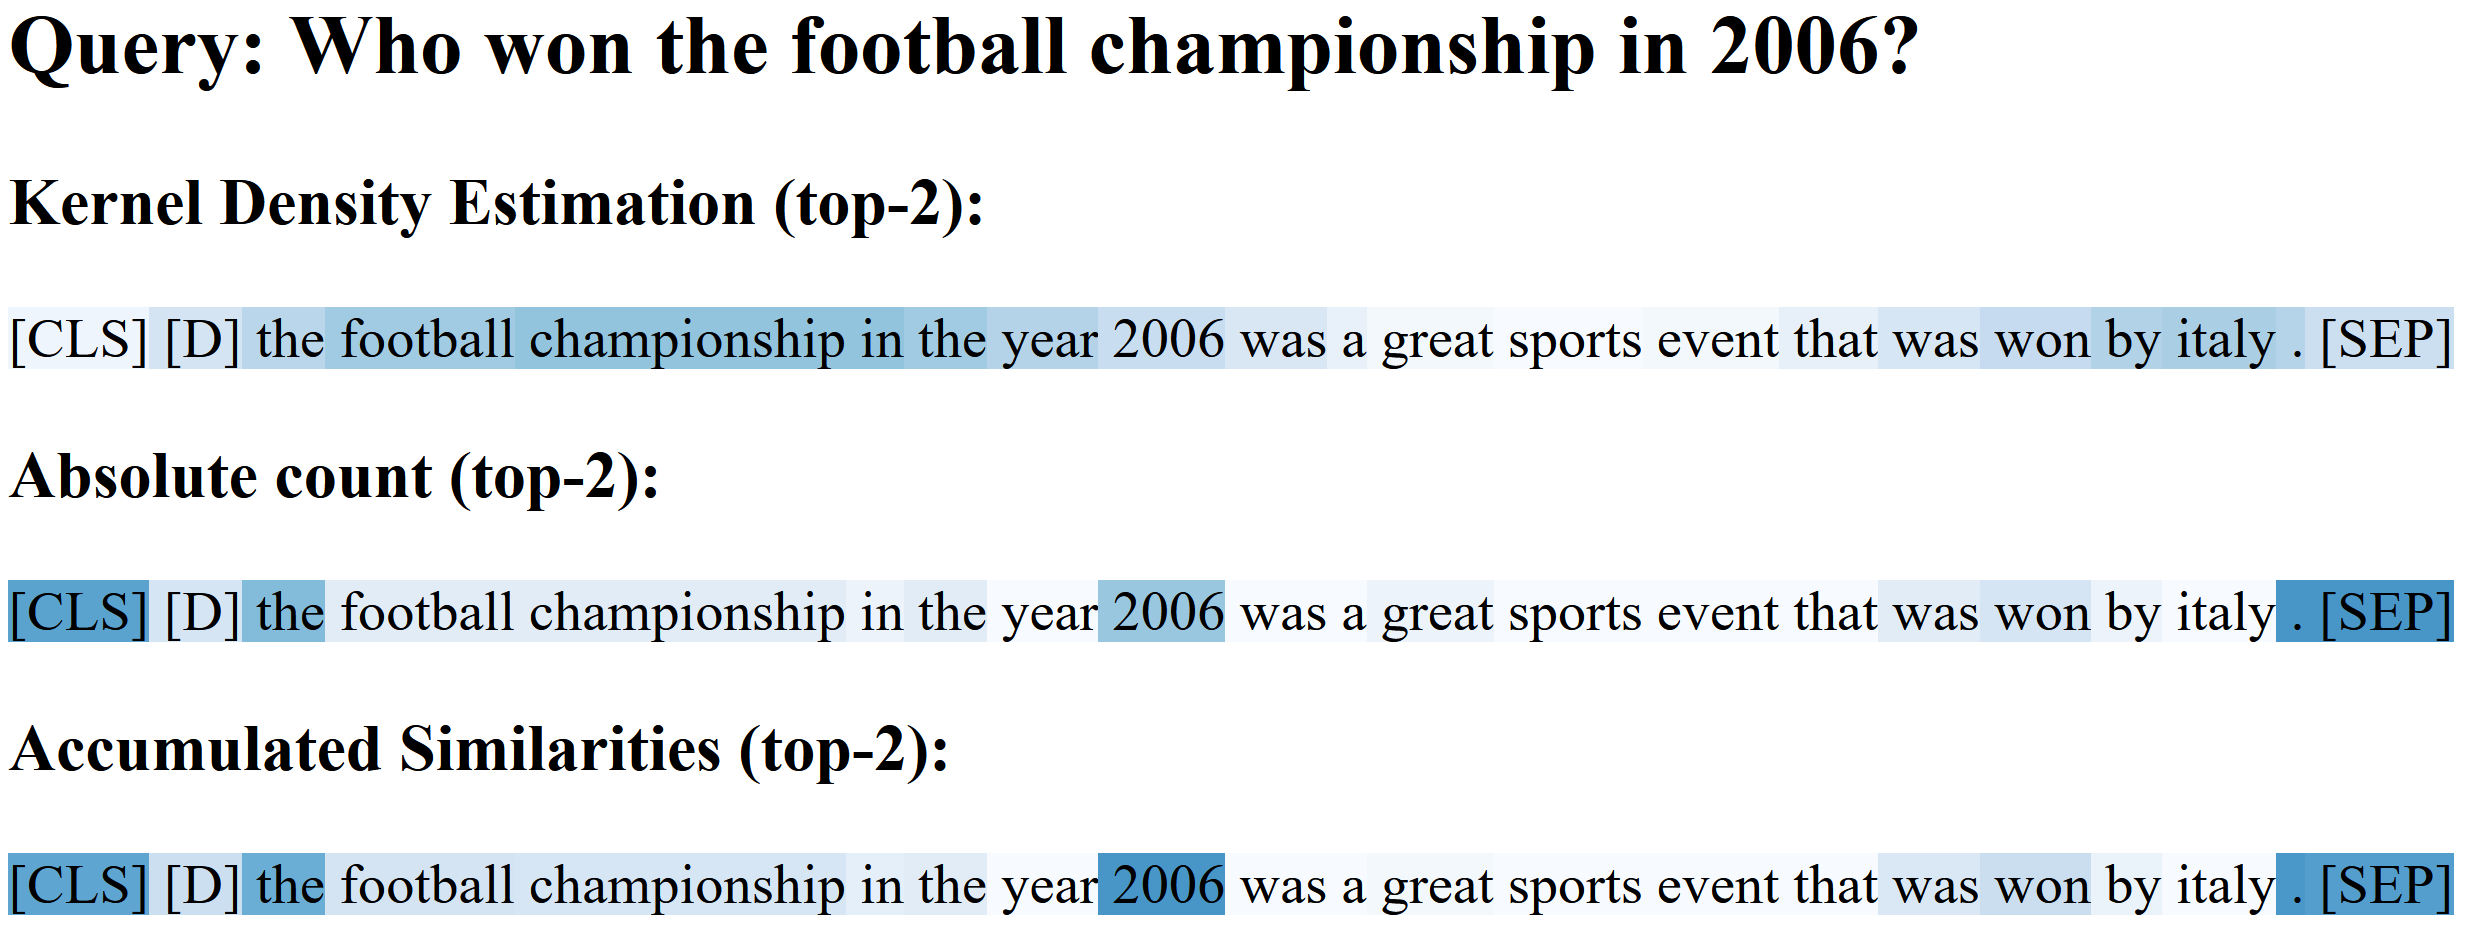
\includegraphics[width = 7.6cm, left]{"./images/heatmap1.png"}
	\caption{KDE, Abs. Count, Acc. Similarities}
	\label{fig:example1}
\end{figure}

ColBERT reliably identifies the passage containing the answer to the given question by comparing the passage embedding with the query embedding. 
However, in most cases, the answer cannot be directly identified by comparing the embedding of the passage with the embedding of the query.
In most instances, the words in the passage that exhibit the highest similarity with the query are not the answer itself, but rather the words 
that lead to the answer.
When comparing the query "Who won the football championship in 2006?" and the passage "The football championship in the year 2006 was a great 
sports event that was won by Italy." of figure~\ref{fig:example1} the highest similarity will be found in the words "the", "football", "championship", "2006", "was", 
"won" and "by" instead  of the actual answer "Italy", because the actual answer is not relevant to decide whether the question is answered 
in the passage. 
ColBERT was not trained to find the answer, but rather to determine whether the answer is contained within the passage.
Substituting any other word for "Italy" would have minimal impact on the probability of the passage providing an answer to the question.
Kernel Density Estimation (KDE) partially addresses this problem by assuming that the answer is likely to be located in the areas of the passage 
that contain a higher concentration of relevant tokens with respect to the question.
The tokens \texttt{[CLS]}, \texttt{[D]} and \texttt{[SEP]} are ignored by KDE.
The markings aid the user in swiftly identifying the likely location of the answer within the passage. Moreover, the markings elucidate the 
significance of the retrieved passage to ColBERT. 
In the event that the answer is not present in the passage, the user can hopefully discern the reasons for ColBERT's failure and
subsequently modify the query accordingly.
 
\begin{figure}[h]
	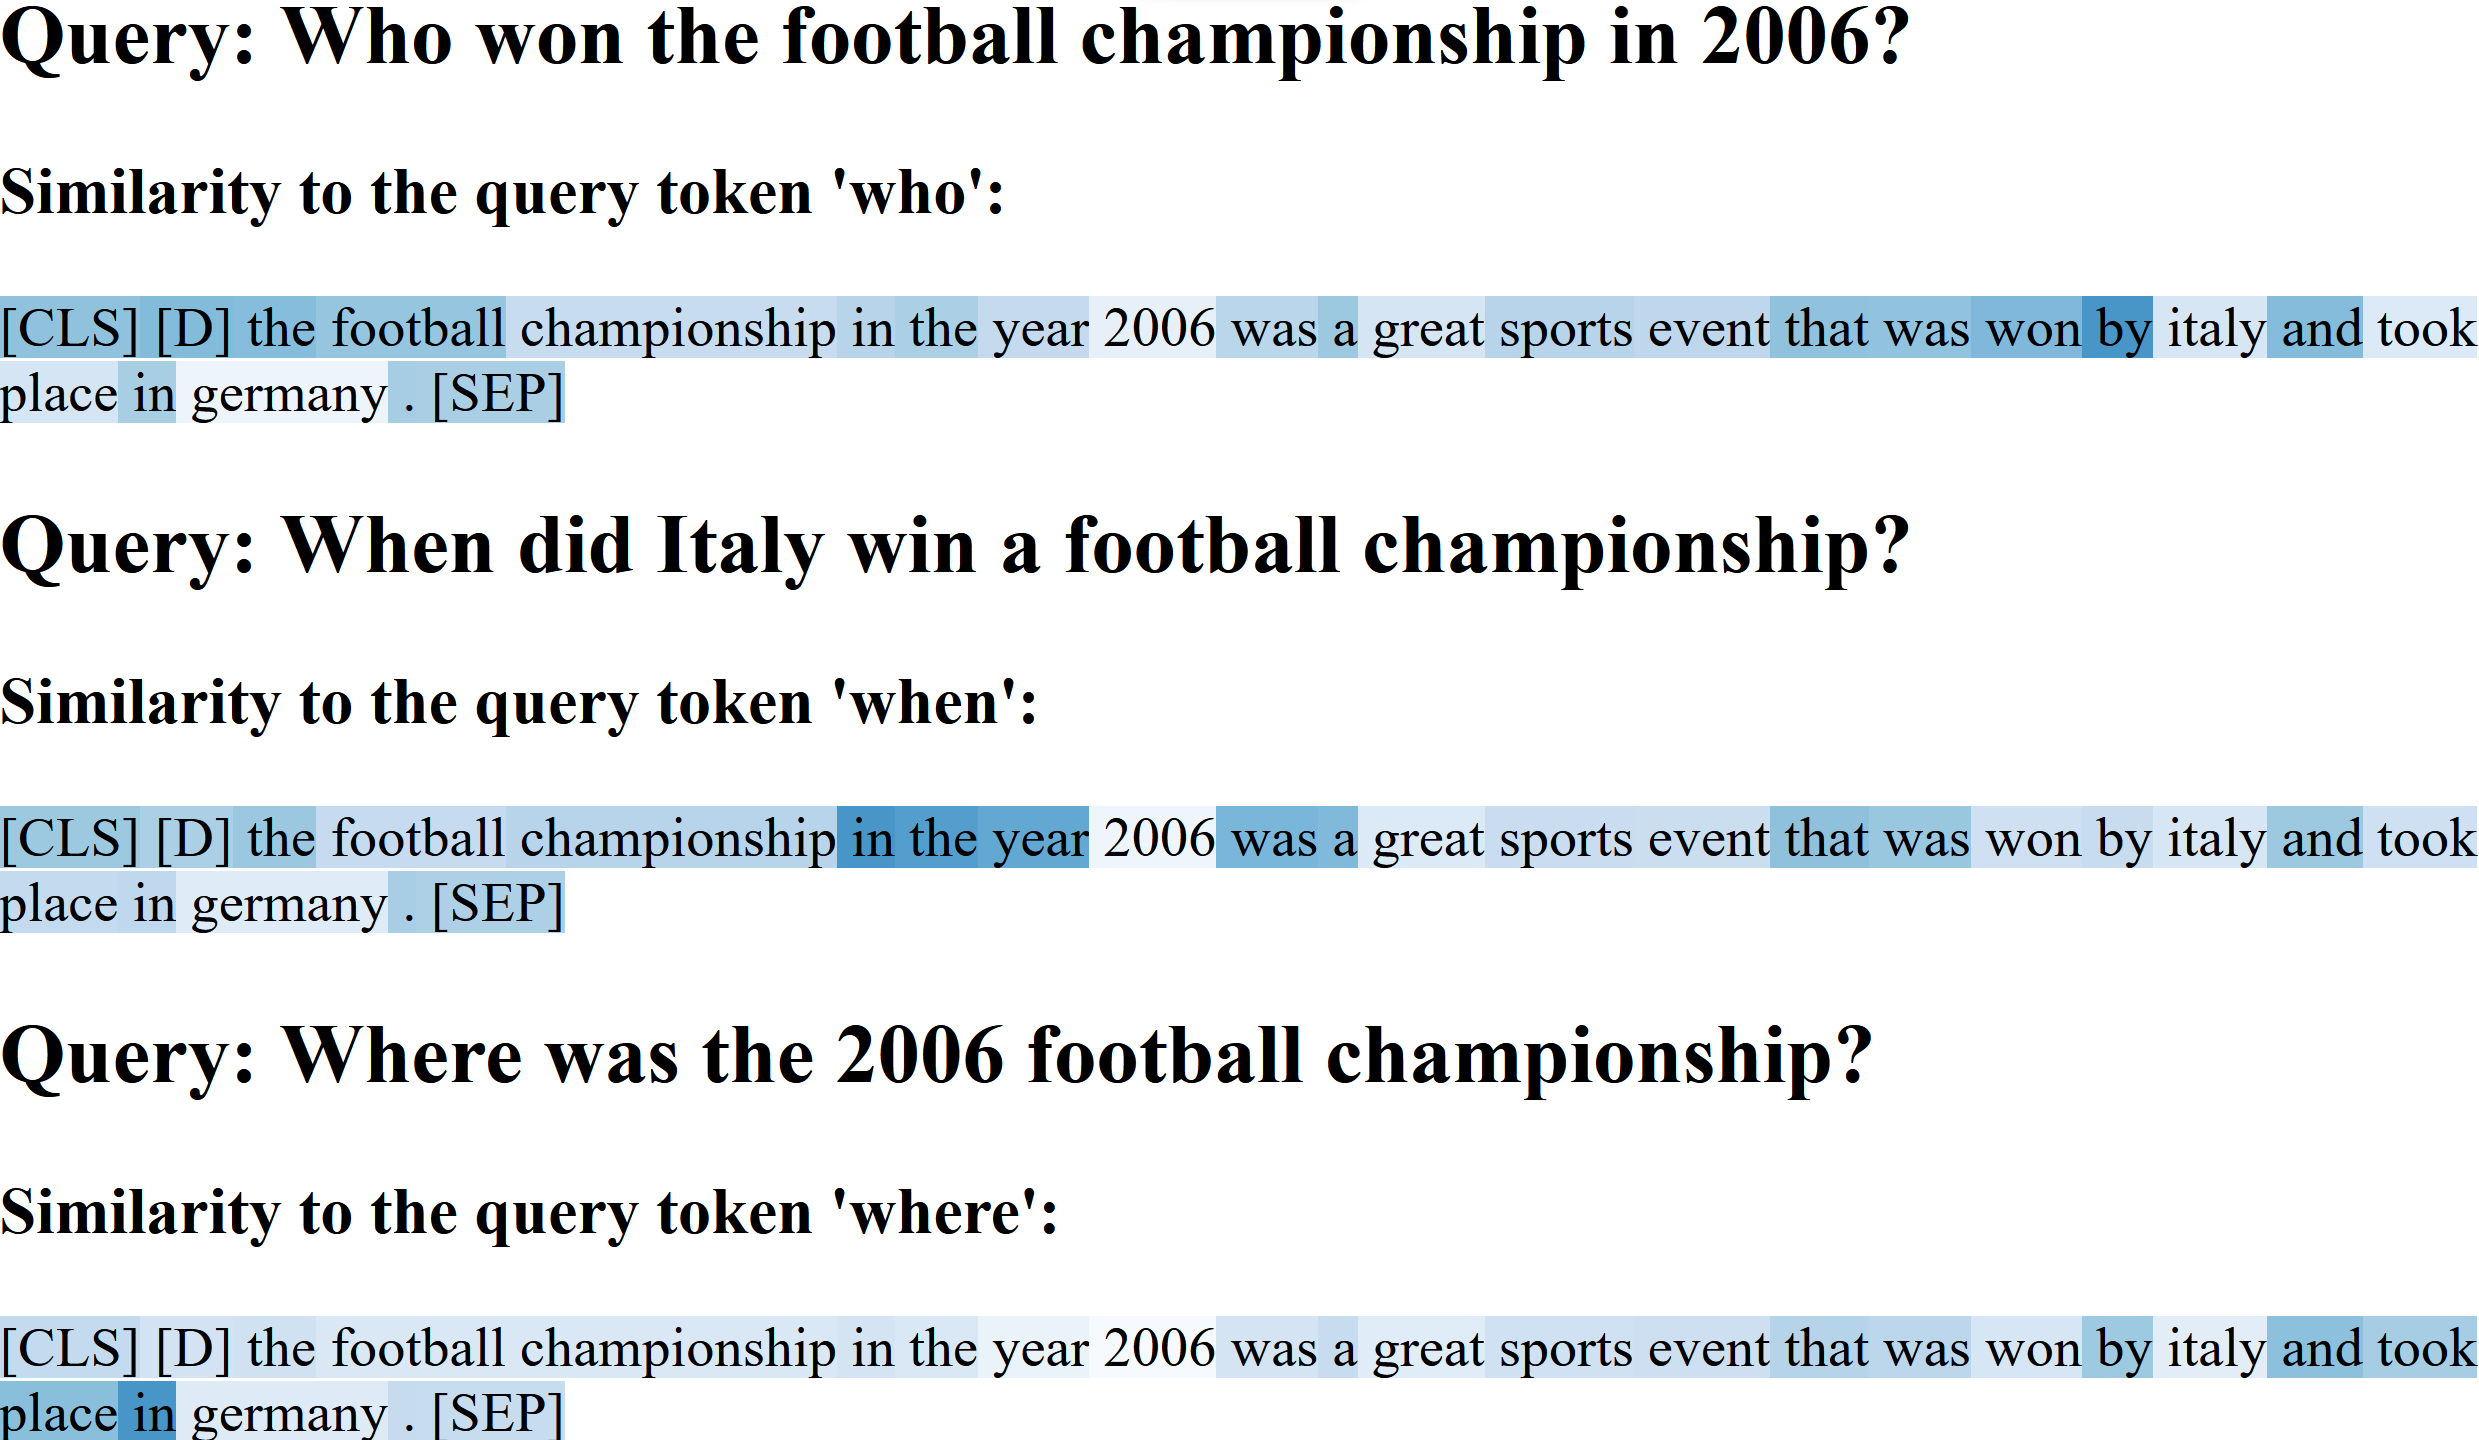
\includegraphics[width = 7.6cm, left]{"./images/first_word_heatmap.png"}
	\caption{Single Token Similarity}
	\label{fig:example2}
\end{figure} 
 
 The major strength of ColBERT lies in its understanding of semantics, where words are not considered in isolation but in context. However, ColBERT encounters similar issues as single-word-based systems like TF-IDF. In Example 2, the similarity for the word 'when' is visualized. Evidently, ColBERT comprehends the intended meaning behind the interrogative word 'when.' Nevertheless, ColBERT often misses the mark in answering the question and instead retrieves passages that provide extensive information about the content of the question. ColBERT is easily distracted by passages that extensively cover the topic of the question. Passages that succinctly provide the answer but have a different core topic are overlooked by ColBERT. Additionally, it seems that insufficient attention is given to the interrogative word.
 This behavior can be explained by the fact that during the training phase, there are only a few passages that contain substantial information about the topic of the question but do not directly answer the question.
 

\section{Introduction}

These instructions are for authors submitting papers to ACL 2023 using \LaTeX. They are not self-contained. All authors must follow the general instructions for *ACL proceedings,\footnote{\url{http://acl-org.github.io/ACLPUB/formatting.html}} as well as guidelines set forth in the ACL 2023 call for papers.\footnote{\url{https://2023.aclweb.org/calls/main_conference/}} This document contains additional instructions for the \LaTeX{} style files.
The templates include the \LaTeX{} source of this document (\texttt{acl2023.tex}),
the \LaTeX{} style file used to format it (\texttt{acl2023.sty}),
an ACL bibliography style (\texttt{acl\_natbib.bst}),
an example bibliography (\texttt{custom.bib}),
and the bibliography for the ACL Anthology (\texttt{anthology.bib}).

\section{Engines}

To produce a PDF file, pdf\LaTeX{} is strongly recommended (over original \LaTeX{} plus dvips+ps2pdf or dvipdf). Xe\LaTeX{} also produces PDF files, and is especially suitable for text in non-Latin scripts.
\begin{table}
\centering
\begin{tabular}{lc}
\hline
\textbf{Command} & \textbf{Output}\\
\hline
\verb|{\"a}| & {\"a} \\
\verb|{\^e}| & {\^e} \\
\verb|{\`i}| & {\`i} \\ 
\verb|{\.I}| & {\.I} \\ 
\verb|{\o}| & {\o} \\
\verb|{\'u}| & {\'u}  \\ 
\verb|{\aa}| & {\aa}  \\\hline
\end{tabular}
\begin{tabular}{lc}
\hline
\textbf{Command} & \textbf{Output}\\
\hline
\verb|{\c c}| & {\c c} \\ 
\verb|{\u g}| & {\u g} \\ 
\verb|{\l}| & {\l} \\ 
\verb|{\~n}| & {\~n} \\ 
\verb|{\H o}| & {\H o} \\ 
\verb|{\v r}| & {\v r} \\ 
\verb|{\ss}| & {\ss} \\
\hline
\end{tabular}
\caption{Example commands for accented characters, to be used in, \emph{e.g.}, Bib\TeX{} entries.}
\label{tab:accents}
\end{table}
\section{Preamble}
\begin{table*}
\centering
\begin{tabular}{lll}
\hline
\textbf{Output} & \textbf{natbib command} & \textbf{Old ACL-style command}\\
\hline
\citep{ct1965} & \verb|\citep| & \verb|\cite| \\
\citealp{ct1965} & \verb|\citealp| & no equivalent \\
\citet{ct1965} & \verb|\citet| & \verb|\newcite| \\
\citeyearpar{ct1965} & \verb|\citeyearpar| & \verb|\shortcite| \\
\citeposs{ct1965} & \verb|\citeposs| & no equivalent \\
\citep[FFT;][]{ct1965} &  \verb|\citep[FFT;][]| & no equivalent\\
\hline
\end{tabular}
\caption{\label{citation-guide}
Citation commands supported by the style file.
The style is based on the natbib package and supports all natbib citation commands.
It also supports commands defined in previous ACL style files for compatibility.
}
\end{table*}
The first line of the file must be
\begin{quote}
\begin{verbatim}
\documentclass[11pt]{article}
\end{verbatim}
\end{quote}
To load the style file in the review version:
\begin{quote}
\begin{verbatim}
\usepackage[review]{ACL2023}
\end{verbatim}
\end{quote}
For the final version, omit the \verb|review| option:
\begin{quote}
\begin{verbatim}
\usepackage{ACL2023}
\end{verbatim}
\end{quote}
To use Times Roman, put the following in the preamble:
\begin{quote}
\begin{verbatim}
\usepackage{times}
\end{verbatim}
\end{quote}
(Alternatives like txfonts or newtx are also acceptable.)
Please see the \LaTeX{} source of this document for comments on other packages that may be useful.
Set the title and author using \verb|\title| and \verb|\author|. Within the author list, format multiple authors using \verb|\and| and \verb|\And| and \verb|\AND|; please see the \LaTeX{} source for examples.
By default, the box containing the title and author names is set to the minimum of 5 cm. If you need more space, include the following in the preamble:
\begin{quote}
\begin{verbatim}
\setlength\titlebox{<dim>}
\end{verbatim}
\end{quote}
where \verb|<dim>| is replaced with a length. Do not set this length smaller than 5 cm.

\section{Document Body}

\subsection{Footnotes}

Footnotes are inserted with the \verb|\footnote| command.\footnote{This is a footnote.}

\subsection{Tables and figures}

See Table~\ref{tab:accents} for an example of a table and its caption.
\textbf{Do not override the default caption sizes.}

\subsection{Hyperlinks}

Users of older versions of \LaTeX{} may encounter the following error during compilation: 
\begin{quote}
\tt\verb|\pdfendlink| ended up in different nesting level than \verb|\pdfstartlink|.
\end{quote}
This happens when pdf\LaTeX{} is used and a citation splits across a page boundary. The best way to fix this is to upgrade \LaTeX{} to 2018-12-01 or later.

\subsection{Citations}



Table~\ref{citation-guide} shows the syntax supported by the style files.
We encourage you to use the natbib styles.
You can use the command \verb|\citet| (cite in text) to get ``author (year)'' citations, like this citation to a paper by \citet{Gusfield:97}.
You can use the command \verb|\citep| (cite in parentheses) to get ``(author, year)'' citations \citep{Gusfield:97}.
You can use the command \verb|\citealp| (alternative cite without parentheses) to get ``author, year'' citations, which is useful for using citations within parentheses (e.g. \citealp{Gusfield:97}).

\subsection{References}

\nocite{Ando2005,augenstein-etal-2016-stance,andrew2007scalable,rasooli-tetrault-2015,goodman-etal-2016-noise,harper-2014-learning}

The \LaTeX{} and Bib\TeX{} style files provided roughly follow the American Psychological Association format.
If your own bib file is named \texttt{custom.bib}, then placing the following before any appendices in your \LaTeX{} file will generate the references section for you:
\begin{quote}
\begin{verbatim}
\bibliographystyle{acl_natbib}
\bibliography{custom}
\end{verbatim}
\end{quote}
You can obtain the complete ACL Anthology as a Bib\TeX{} file from \url{https://aclweb.org/anthology/anthology.bib.gz}.
To include both the Anthology and your own .bib file, use the following instead of the above.
\begin{quote}
\begin{verbatim}
\bibliographystyle{acl_natbib}
\bibliography{anthology,custom}
\end{verbatim}
\end{quote}
Please see Section~\ref{sec:bibtex} for information on preparing Bib\TeX{} files.

\subsection{Appendices}

Use \verb|\appendix| before any appendix section to switch the section numbering over to letters. See Appendix~\ref{sec:appendix} for an example.

\section{Bib\TeX{} Files}
\label{sec:bibtex}

Unicode cannot be used in Bib\TeX{} entries, and some ways of typing special characters can disrupt Bib\TeX's alphabetization. The recommended way of typing special characters is shown in Table~\ref{tab:accents}.

Please ensure that Bib\TeX{} records contain DOIs or URLs when possible, and for all the ACL materials that you reference.
Use the \verb|doi| field for DOIs and the \verb|url| field for URLs.
If a Bib\TeX{} entry has a URL or DOI field, the paper title in the references section will appear as a hyperlink to the paper, using the hyperref \LaTeX{} package.

\section*{Limitations}
ACL 2023 requires all submissions to have a section titled ``Limitations'', for discussing the limitations of the paper as a complement to the discussion of strengths in the main text. This section should occur after the conclusion, but before the references. It will not count towards the page limit.
The discussion of limitations is mandatory. Papers without a limitation section will be desk-rejected without review.

While we are open to different types of limitations, just mentioning that a set of results have been shown for English only probably does not reflect what we expect. 
Mentioning that the method works mostly for languages with limited morphology, like English, is a much better alternative.
In addition, limitations such as low scalability to long text, the requirement of large GPU resources, or other things that inspire crucial further investigation are welcome.

\section*{Ethics Statement}
Scientific work published at ACL 2023 must comply with the ACL Ethics Policy.\footnote{\url{https://www.aclweb.org/portal/content/acl-code-ethics}} We encourage all authors to include an explicit ethics statement on the broader impact of the work, or other ethical considerations after the conclusion but before the references. The ethics statement will not count toward the page limit (8 pages for long, 4 pages for short papers).

\section*{Acknowledgements}
This document has been adapted by Jordan Boyd-Graber, Naoaki Okazaki, Anna Rogers from the style files used for earlier ACL, EMNLP and NAACL proceedings, including those for
EACL 2023 by Isabelle Augenstein and Andreas Vlachos,
EMNLP 2022 by Yue Zhang, Ryan Cotterell and Lea Frermann,
ACL 2020 by Steven Bethard, Ryan Cotterell and Rui Yan,
ACL 2019 by Douwe Kiela and Ivan Vuli\'{c},
NAACL 2019 by Stephanie Lukin and Alla Roskovskaya, 
ACL 2018 by Shay Cohen, Kevin Gimpel, and Wei Lu, 
NAACL 2018 by Margaret Mitchell and Stephanie Lukin,
Bib\TeX{} suggestions for (NA)ACL 2017/2018 from Jason Eisner,
ACL 2017 by Dan Gildea and Min-Yen Kan, NAACL 2017 by Margaret Mitchell, 
ACL 2012 by Maggie Li and Michael White, 
ACL 2010 by Jing-Shin Chang and Philipp Koehn, 
ACL 2008 by Johanna D. Moore, Simone Teufel, James Allan, and Sadaoki Furui, 
ACL 2005 by Hwee Tou Ng and Kemal Oflazer, 
ACL 2002 by Eugene Charniak and Dekang Lin, 
and earlier ACL and EACL formats written by several people, including
John Chen, Henry S. Thompson and Donald Walker.
Additional elements were taken from the formatting instructions of the \emph{International Joint Conference on Artificial Intelligence} and the \emph{Conference on Computer Vision and Pattern Recognition}.

% Entries for the entire Anthology, followed by custom entries
% \bibliography{anthology,custom}
\bibliography{custom}
\bibliographystyle{acl_natbib}

\appendix

\section{Example Appendix}
\label{sec:appendix}

This is a section in the appendix.

\end{document}
